\documentclass{article}
\usepackage{graphicx} 
\usepackage{float}
\title{pyMAP start guide}
\author{Aly Aly}
\date{March 2023}

\begin{document}

\maketitle

\section{Purpose}
This is a document to help users get up and running with pyMAP. pyMAP is a set of python programs and Jupyter Notebooks developed to help organize and standardize data analysis tools and database mangement for data associated with IMAP-Lo calibrations and cross calibrations.

\section{ Overview}

This document will cover the process from getting the neccassary application and installing them, to using some notebooks to get and plot data. The list below gives a general outline of steps to be covered. If you are already familiar with some of the steps please feel free to skip around.


Note:\textit{To access the database you will need to be on campus or logged in to the school VPN. For instructions on setting up the VPN please visit https://networking.unh.edu/vpn/}
\begin{enumerate}
    \item Install Anaconda.
    \item Download repository.
    \item Load environment into anaconda.
    \item Use Jupyter notebooks
    \item Special instructions for database access to data from pyMAP
\end{enumerate}

\section{Install Anaconda}
\label{sec:conda_inst}
To download anaconda go to \textit{https://www.anaconda.com/}. The site should detect your operating system. Click on download.
\begin{figure}[H]
\centering
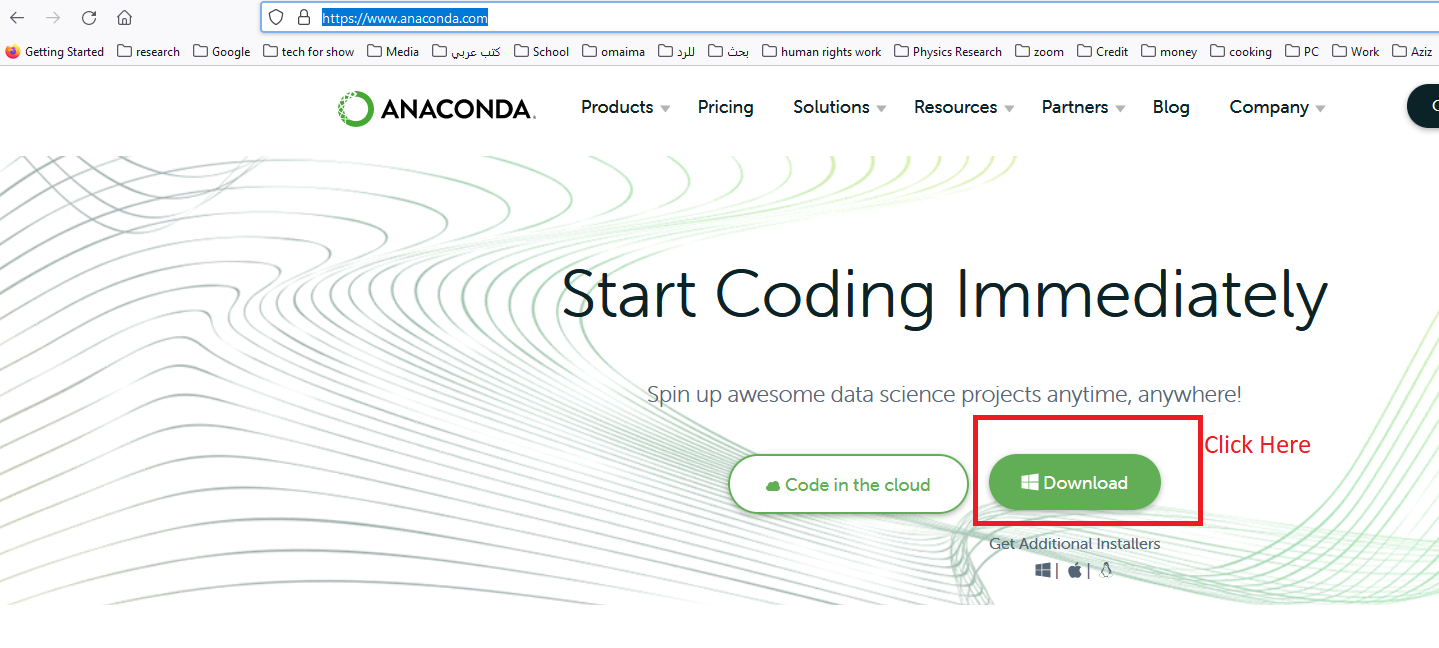
\includegraphics[scale=0.4]{conda_DOWNLOAD.png}
\caption{From www.anaconda.com}
\label{fig:conda_download}
\end{figure}


Once download is complete launch by double clicking on the downloaded file. The installation instructions should be easy to follow and the recommend settings are sufficient to get started. After installation is complete, make sure you have a new icon in your start menu or applications directory.


\section{Download The GIT Repository}
\label{sec:git_inst}
To get a copy of the repository to use for data analysis, it is sufficient to download a zip file. If you are planning on doing development then you should use github to clone and the repository and make pull requests often. To get a copy of the repository go to$ \textit{https://github.com/jonbowr/pyMAP}$ and click on the code menu. Download the repository and unzip the contents in your preferred working directory but you need to call it pyMAP.

\begin{figure}[H]
\centering
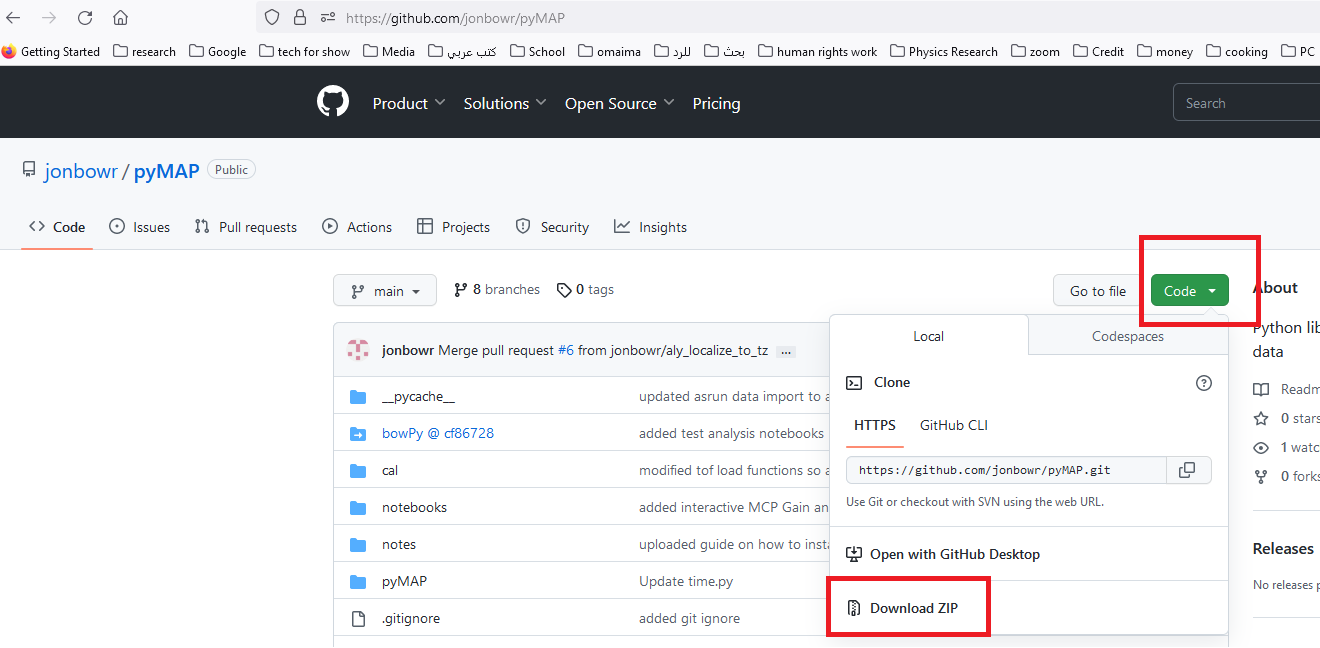
\includegraphics[scale=0.4]{gitdown1.png}
\caption{From \textit{https://github.com/jonbowr/pyMAP}}
\label{fig:git_download1}
\end{figure}


You now have a directory called pyMAP where you unzipped the downloaded git repository. The contents are shown in Figure \ref{fig:git_download2}.


\begin{figure}[H]
\centering
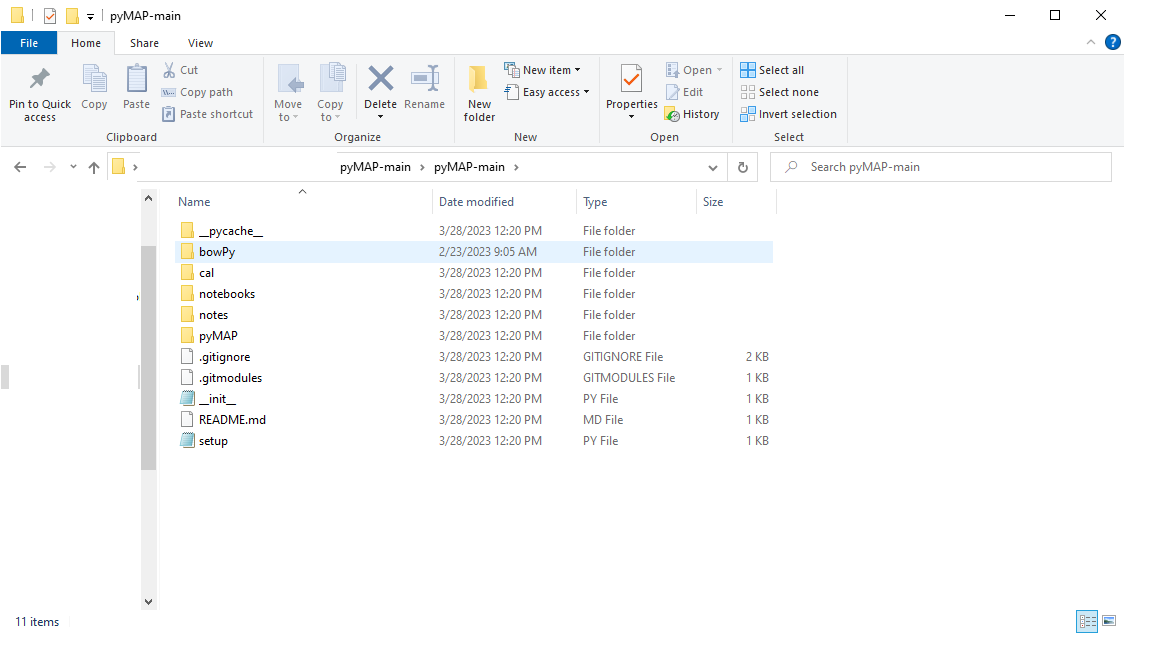
\includegraphics[scale=0.4]{gitdown2.png}
\label{fig:git_download2}
\caption{ Shows the contents of pyMAP repository downloaded as a zipped directory called pyMAP-main which you should change to pyMAP .}
\end{figure}


You are now ready to use the tools in the packages contained in the repository. 


\section{Load The Anaconda Environment}
To load the Anaconda environment one has several options.
\subsection{From Anaconda Navigator}
The Anaconda install leaves you with a new directory containing the Anaconda navigator. launch the navigator(see Figure \ref{fig:load_env1}).

\begin{figure}[H]
\centering
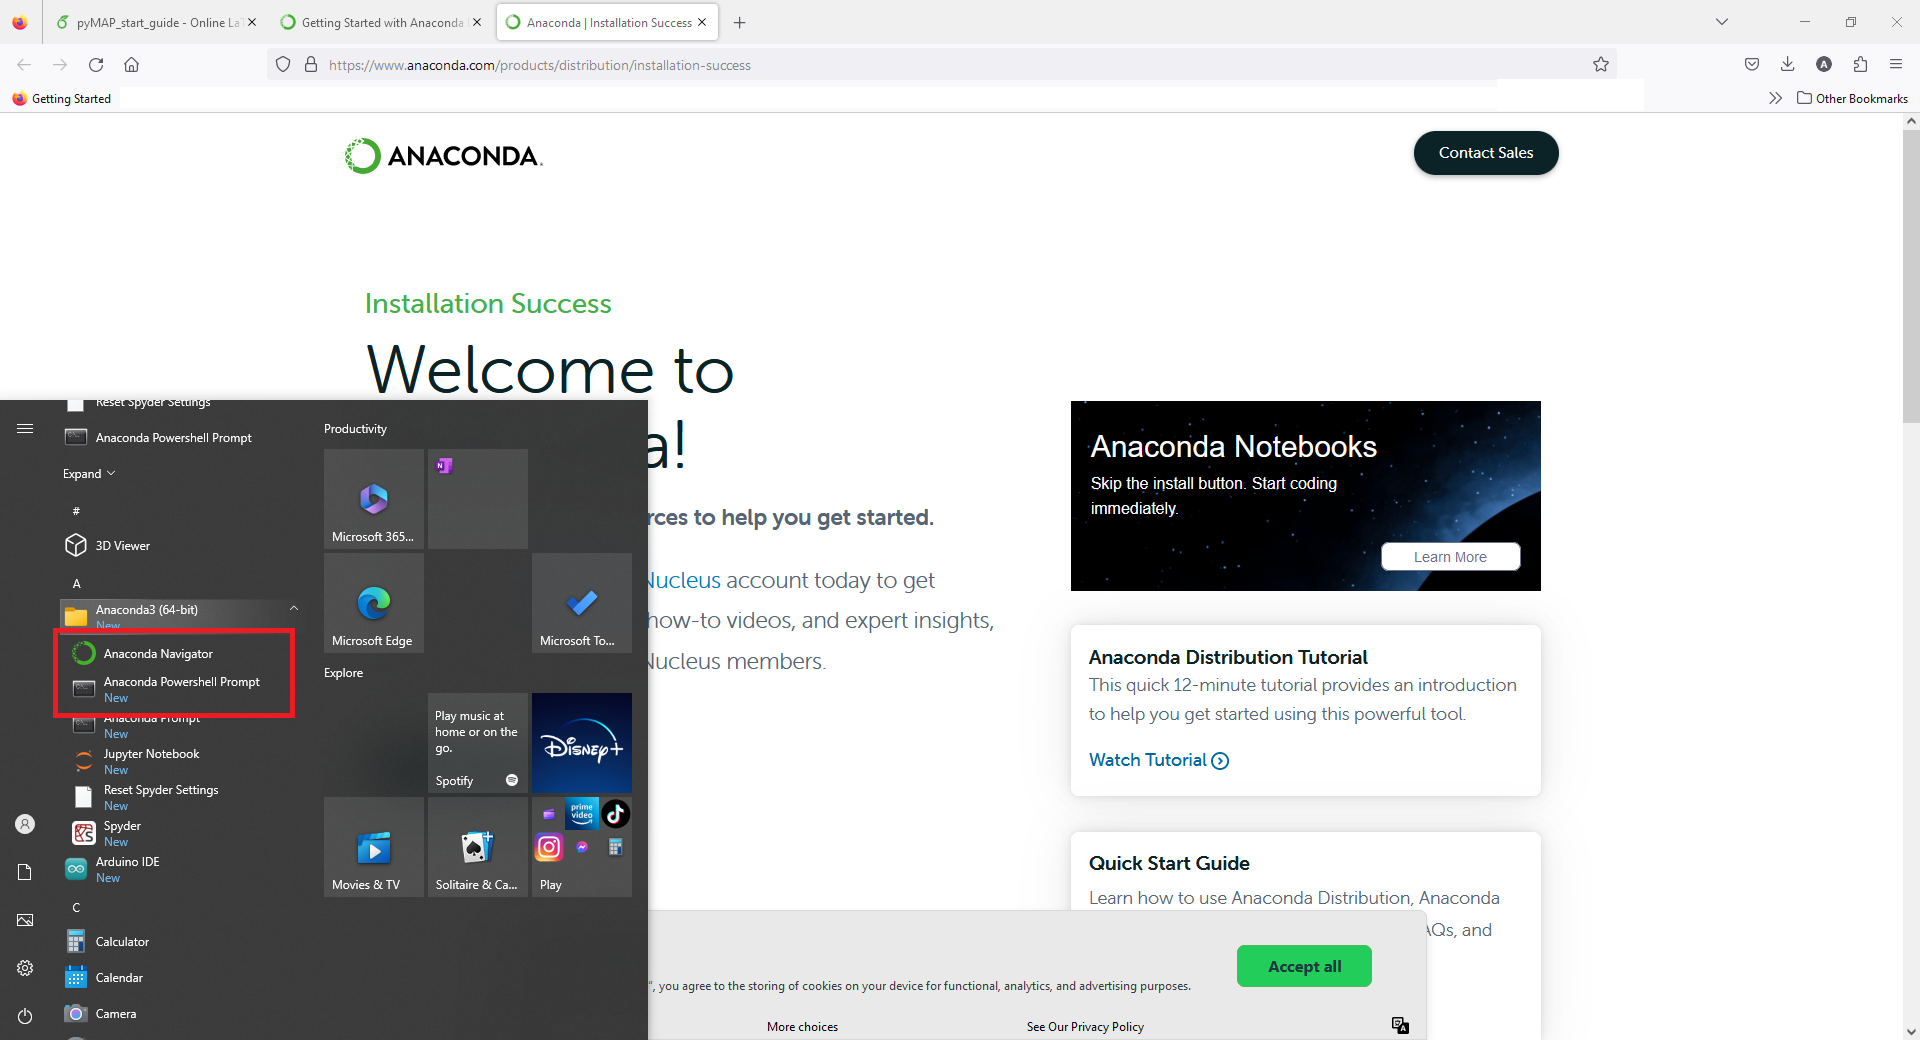
\includegraphics[scale=0.4]{load_env1.png}
\label{fig:load_env1}
\caption{ Shows the contents of Anaconda folder in Windows start menu with navigator and powershell outlined in red.}
\end{figure}

You then add the environment by navigating to the Environments tab outline by a red box labeled 1, in Figure \ref{fig:load_env2}. Click import labeled 2 and select the folder icon next LocalDrive and navigate to the location of the git repository folder and select the \textbf{pyMAP Env.yaml} file (see Figure \ref{fig:load_env3}).

\begin{figure}[H]
\centering
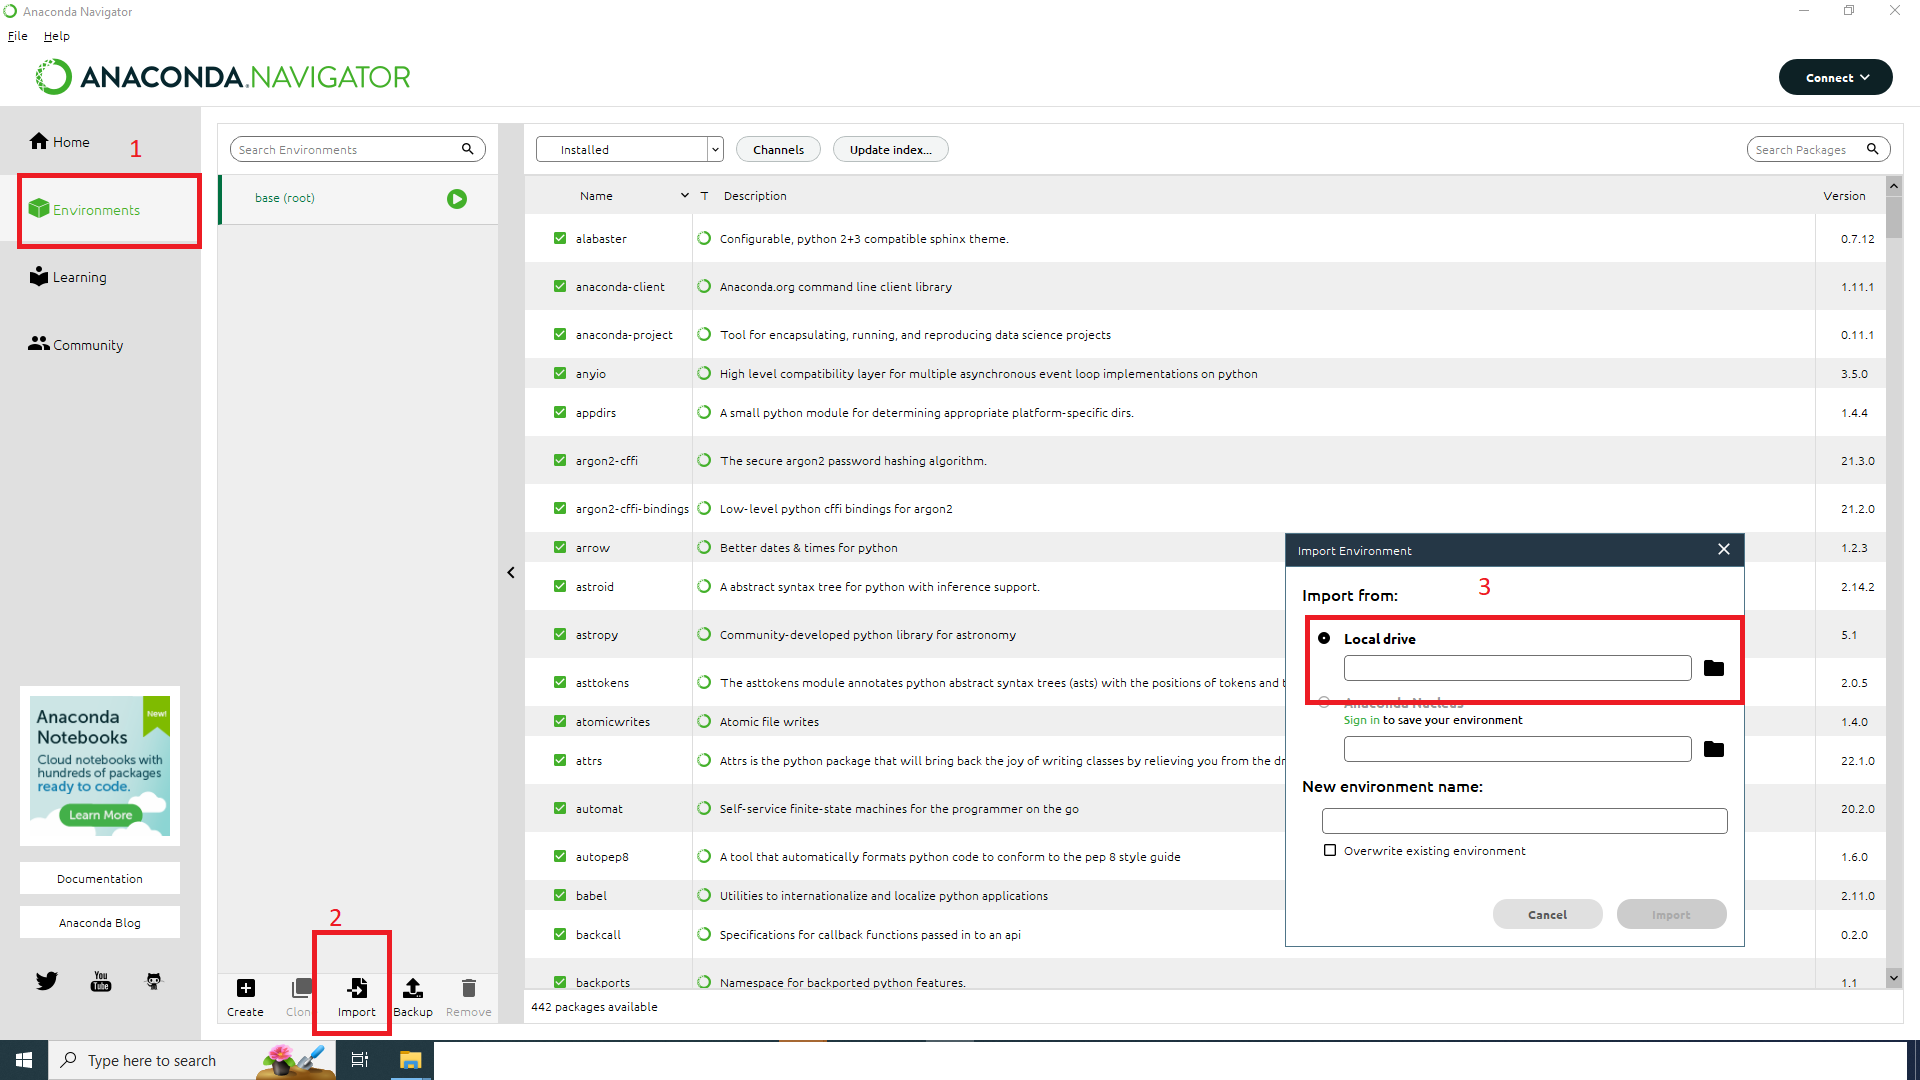
\includegraphics[scale=0.4]{load_env2.png}
\label{fig:load_env2}
\caption{ Shows the Environments tab in red box 1, with the import button in red box 2 and the location popup in red box 3.}
\end{figure}


 


 \begin{figure}[H]
\centering
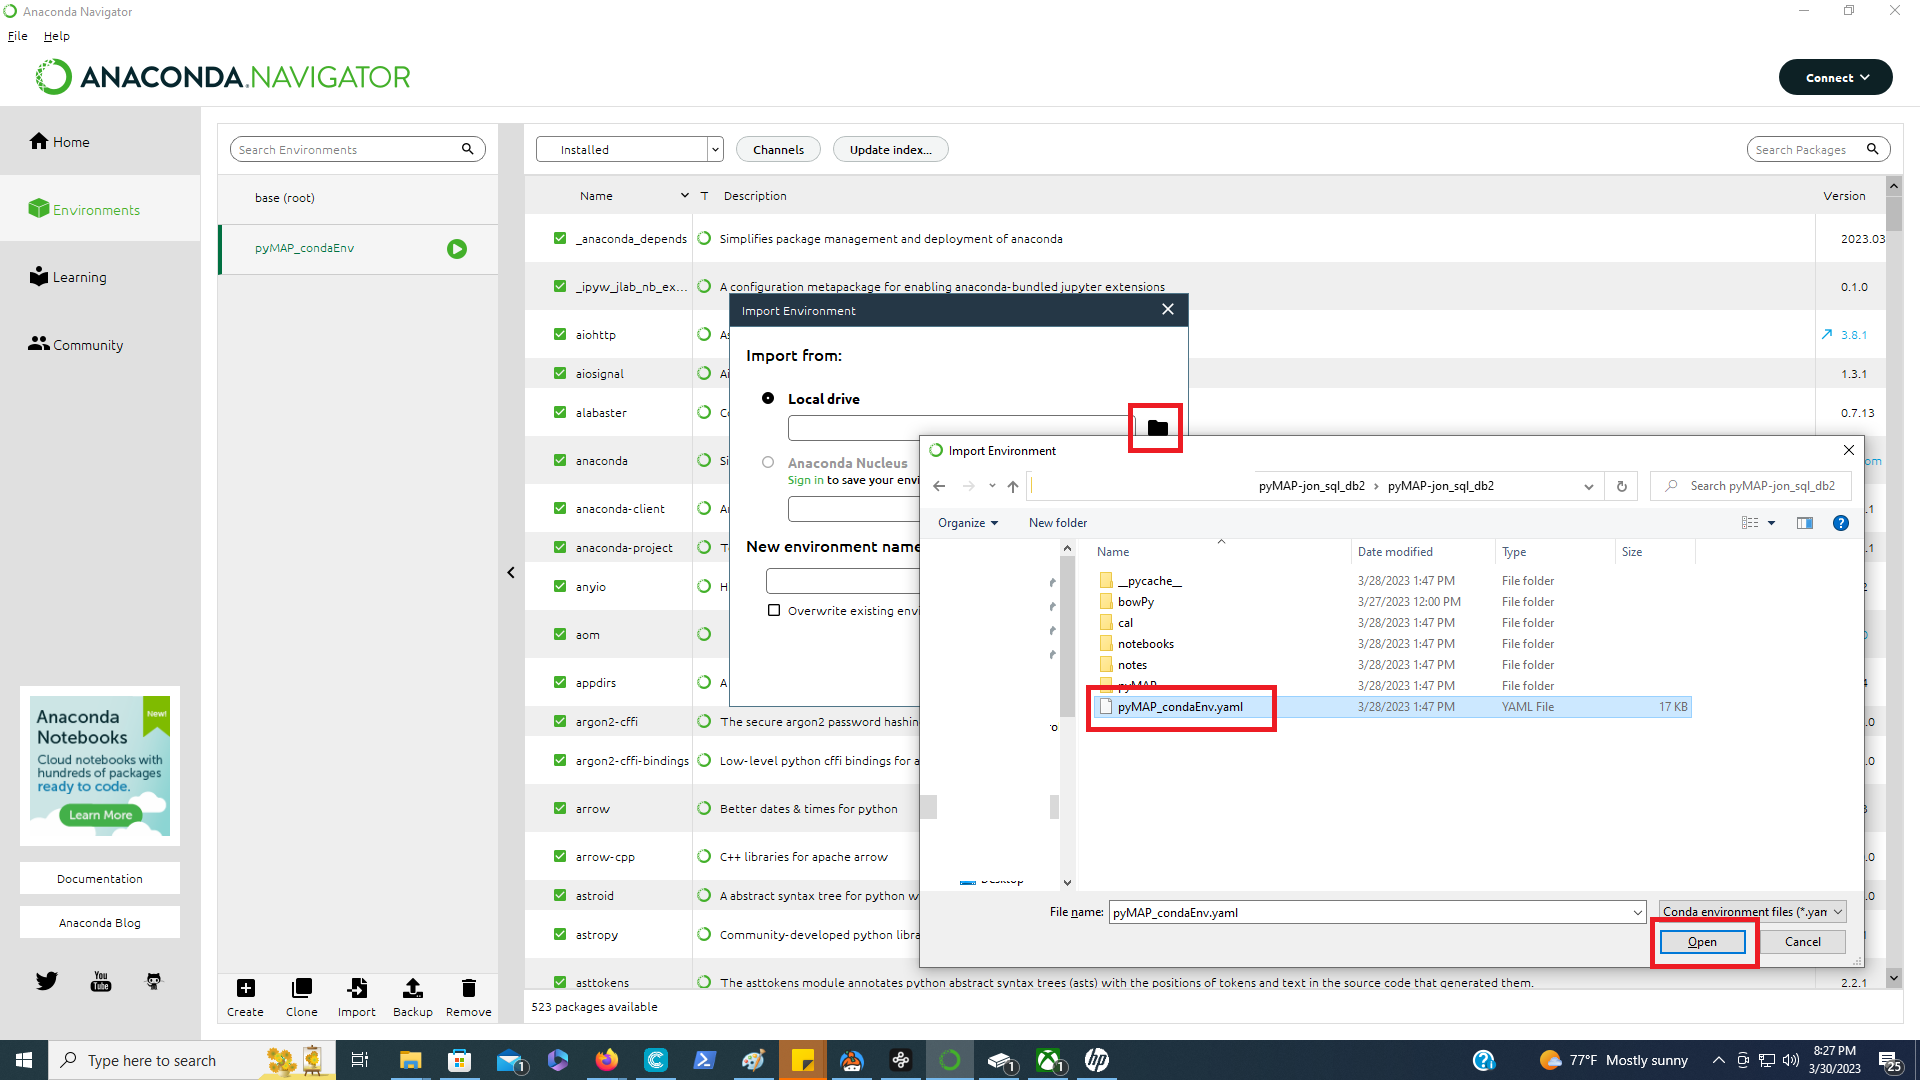
\includegraphics[scale=0.4]{load_env3.png}
\label{fig:load_env3}
\caption{ Shows the Environments tab with the brows icon in small red box.}
\end{figure}


 The environment will take some time to load. This is because new python packages are being installed by Anaconda. 


 You can now go back to the Home tab and launch Jupyter.

 \subsection{From Anaconda Navigator}
 Another way to access packages managed in an Anaconda virtual environment is to activate the  \textbf{pyMAP condaEnv.yaml} in the Anaconda Powershell. This process is much quicker and requires fewer steps. 

 First launch the Anaconda Powershell (see Figure \ref{fig:load_env1}). Once the terminal loads change the current directory to the repository from Section \ref{sec:git_inst} with the cd command. \\

 \textbf{cd Path/to/repository/}

 Next we want to let Anaconda load our environment, \\ \\
\small{
 \textbf{ conda env create --name  ""NameToUseOnThisMachine"" --file=""NameOfEnviornment.ymal""}} \\

, where you need to replace the text in double quotes. \\ \\

Now that Anaconda has loaded your environment you can activate it using: \\ \\
\textbf{conda activate  ""NameToUseOnThisMachine"" } \\ \\

 , and you're ready to launch Jupyter.


 \section{Using Jupyter Notebooks}

 For our analysis tools, we use Jupyter Notebooks which can be launched from the navigator home page or from the Powershell by supplying the command "jupyter notebook". When the application is launched initially no content will appear in the editor pane. you can now use the Notebooks by placing them in the parent folder to the pyMAP directory where you unzipped the github repository from Section \ref{sec:git_inst}. To see how this works we will go through two examples. 

\subsection{Simple SQL Query}
The downloaded repository should come with a "notebooks" directory which had a notebook called 
\end{document}



 